\documentclass[a4paper]{article}
\usepackage{a4wide,amssymb,epsfig,latexsym,multicol,array,hhline,fancyhdr}
\usepackage{amsmath}
\usepackage{lastpage}
\usepackage[lined,boxed,commentsnumbered]{algorithm2e}
\usepackage{enumerate}
\usepackage{color}
\usepackage{graphicx}							% Standard graphics package
\usepackage{array}
\usepackage{tabularx, caption}
\usepackage{multirow}
\usepackage{multicol}
\usepackage{rotating}
\usepackage{graphics}
\usepackage{geometry}
\usepackage{setspace}
\usepackage{epsfig}
\usepackage{enumitem}
\usepackage{float}
\usepackage{caption}  
\usepackage{indentfirst}

% Required packages and libraries
\usepackage{tikz}
\usetikzlibrary{petri,positioning}
\usetikzlibrary{shapes.geometric}
\usetikzlibrary{automata,positioning,arrows}
\usepackage[utf8]{inputenc}
\usepackage[english]{babel}
\usepackage{hyperref}
\hypersetup{urlcolor=blue,linkcolor=black,citecolor=black,colorlinks=true} 
%\usepackage{pstcol} 								% PSTricks with the standard color package

\newtheorem{theorem}{{\bf Theorem}}
\newtheorem{property}{{\bf Property}}
\newtheorem{proposition}{{\bf Proposition}}
\newtheorem{corollary}[proposition]{{\bf Corollary}}
\newtheorem{lemma}[proposition]{{\bf Lemma}}

\AtBeginDocument{\renewcommand*\contentsname{Contents}}
\AtBeginDocument{\renewcommand*\refname{References}}
%\usepackage{fancyhdr}
\setlength{\headheight}{40pt}
\pagestyle{fancy}
\fancyhead{} % clear all header fields
\fancyhead[L]{
 \begin{tabular}{rl}
    \begin{picture}(25,15)(0,0)
    \put(0,-8){\includegraphics[width=8mm, height=8mm]{hcmut.png}}
    %\put(0,-8){\epsfig{width=10mm,figure=hcmut.eps}}
   \end{picture}&
	%\includegraphics[width=8mm, height=8mm]{hcmut.png} & %
	\begin{tabular}{l}
		\textbf{\bf \ttfamily University of Technology, Ho Chi Minh City}\\
		\textbf{\bf \ttfamily Faculty of Computer Science and Engineering}
	\end{tabular} 	
 \end{tabular}
}
\fancyhead[R]{
	\begin{tabular}{l}
		\tiny \bf \\
		\tiny \bf 
	\end{tabular}  }
\fancyfoot{} % clear all footer fields
\fancyfoot[L]{\scriptsize \ttfamily Assignment for Discrete Mathematics - Academic year 2020 - 2021}
\fancyfoot[R]{\scriptsize \ttfamily Page {\thepage}/\pageref{LastPage}}
\renewcommand{\headrulewidth}{0.3pt}
\renewcommand{\footrulewidth}{0.3pt}


%%%
\setcounter{secnumdepth}{4}
\setcounter{tocdepth}{3}
\makeatletter
\newcounter {subsubsubsection}[subsubsection]
\renewcommand\thesubsubsubsection{\thesubsubsection .\@alph\c@subsubsubsection}
\newcommand\subsubsubsection{\@startsection{subsubsubsection}{4}{\z@}%
                                     {-3.25ex\@plus -1ex \@minus -.2ex}%
                                     {1.5ex \@plus .2ex}%
                                     {\normalfont\normalsize\bfseries}}
\newcommand*\l@subsubsubsection{\@dottedtocline{3}{10.0em}{4.1em}}
\newcommand*{\subsubsubsectionmark}[1]{}
%paragraph indentation
\setlength{\parindent}{4em} 

%paragraph spacing
\setlength{\parskip}{0.5em}
\usetikzlibrary{arrows.meta,positioning}

%Line spacing
\renewcommand{\baselinestretch}{1.5}
\begin{document}
\begin{titlepage}
	\begin{center}
		VIETNAM NATIONAL UNIVERSITY, HO CHI MINH CITY \\
		UNIVERSITY OF TECHNOLOGY \\
		FACULTY OF COMPUTER SCIENCE AND ENGINEERING
	\end{center}

	\vspace{1cm}

	\begin{figure}[h!]
		\begin{center}
			\includegraphics[width=3cm]{hcmut.png}
		\end{center}
	\end{figure}

	\vspace{1cm}


	\begin{center}
		\begin{tabular}{c}
			\multicolumn{1}{c}{\textbf{{\Large DISCRETE MATHEMATICS }}} \\
			~~                                                                   \\
			\hline
			\\
			\textbf{{\Huge ASSIGNMENT REPORT}}                               \\
			\\
			\hline
		\end{tabular}
	\end{center}

	\vspace{2cm}

	\begin{table}[h]
		\begin{tabular}{rrl}
			\hspace{5 cm} & Advisor:  &          \\
			              & Students: &  \\
			              &           &         \\
		\end{tabular}
	\end{table}

	\begin{center}
		{\footnotesize HO CHI MINH CITY, NOVEMBER 2021}
	\end{center}
\end{titlepage}


%\thispagestyle{empty}

\newpage
\tableofcontents
\newpage


%%%%%%%%%%%%%%%%%%%%%%%%%%%%%%%%%
\section{Member list \& Workload}

\begin{center}
	\begin{tabular}{|c|c|c|l|c|}
		\hline
		\textbf{No.}       & \textbf{Fullname}                    & \textbf{Student ID}      & \textbf{Problems}                 & \textbf{Percentage of work} \\
		\hline
		%%%%%Student 1%%%%%%%%%%
		\multirow{3}{*}{1} & \multirow{3}{*}{} & \multirow{3}{*}{} & - Text                            & \multirow{3}{*}{40\%}       \\
		                   &                                      &                          & Text.                             &                             \\
		                   &                                      &                          & - Text.                           &                             \\
		\hline
		%%%%%Student 2%%%%%%%%%%%
		\multirow{3}{*}{2} & \multirow{3}{*}{}        & \multirow{3}{*}{} & - Relation \& Counting: 4, 5, 6   & \multirow{3}{*}{20\%}       \\
		                   &                                      &                          & Bonus: 4, 5, 6.                   &                             \\
		                   &                                      &                          & - Graph: 1, 2, 3, Bonus: 1, 2, 3. &                             \\
		\hline
	\end{tabular}
\end{center}
\newpage
%%%%%%%%%%%%%%%%%%%%%%%%%%%%%%%%%
\section{Introduction To Assignment}
\par
We will discuss several common problems such as Shortest-Path Algorithms and Network Flow Problem in graph theory in this report. Not only are these
algorithms useful in practice, they are also interesting because in many real-life applications.
\par
%%%%%%%%%%%%%%%%%%%%%%%%%%%%%%%%%
\section{Solving Assignment Problem}
\subsection{Problem 1}
\subsubsection{Kth Shortest Path Algorithm}
\subsubsubsection{Algorithm}
\par
The idea is using DFS (Deep-First Search) algorithm to find all possible paths from the source to the destination and adding loops to path if graph contains loops then storing them in the array.
Then we will calculate the length of each path and sort them in ascending order. The k-th shortest path is the k-th element in the sorted array.\\
Example:
\begin{figure}[H]
	\centering
	\begin{tikzpicture}[node distance=3cm,on grid]

		% Place 1
		\node[place,
			fill=orange!25,
			draw=orange!75] (place1) {0};
		
		% Place 2
		\node[place,
			fill=orange!25,
			draw=orange!75,
			right = 2cm of place1] (place2) {3};
		
		% Place 3
		\node[place,
			fill=orange!25,
			draw=orange!75,
			below = 2cm of place1] (place3) {1};
		% Place 4
		\node[place,
			fill=orange!25,
			draw=orange!75,
			below left = 1cm and 2cm of place1] (place4) {2};
		\draw[thick] (place1) edge[post] node[sloped, anchor=center, above] {2} (place2)
		(place1) edge[post] node[align=center, anchor=center, left] {1} (place3)
		(place1) edge[post, bend right = 20] node[sloped, anchor=center, above] {3} (place4)
		(place4) edge[post, bend right = 20] node[sloped, anchor=center, below] {1} (place1)
		(place4) edge[post] node[sloped, anchor=center, below] {3}  (place3)
		(place3) edge[post] node[sloped, anchor=center, below] {4} (place2)
		(place4) edge[loop above] node[sloped, anchor=center, above] {6} (place4)
		;
	\end{tikzpicture}
	\caption{Print 2nd Shortest Path from 2 to 3} 
	\label{fig:q1}
\end{figure}
\par We set the THRESHOLD to be 3, which means we will only consider the paths with the maximum loop length less than 3.
After running the algorithm, we will get the following paths (We consider several paths): 
\begin{itemize}
	\item {2, 0, 1, 3} Length: 6
	\item {2, 0, 3} Length: 3
	\item {2, 1, 3} Length: 7
	\item {2, 2, 0, 1, 3} Length: 12
\end{itemize}
Then we sort the paths in ascending order and get the resulting paths from the sorted array:
\begin{itemize}
	\item {2, 0, 3} Length: 3
	\item {2, 0, 1, 3} Length: 6
	\item {2, 1, 3} Length: 7
	\item {2, 2, 0, 1, 3} Length: 12
\end{itemize}
So the second Shortest Path from 2 to 3 is the path {2, 0, 1, 3} with length 6.
\subsubsubsection{Code Input}

\begin{figure}[H]\centering
	\includegraphics[width= 8 cm]{QUES1A.png}
	\caption{Input for example in Problem 1a}
\end{figure}
\subsubsection{Kth Shortest Path Without Loops}
\subsubsubsection{Algorithm}

\par
By using DFS algorithm and mark visited node, we can find the shortest path from the source to the destination without loops.\\
From the example of Fig.~\ref{fig:q1}, we get three shortest paths without loops from the source to the destination:
\begin{itemize}
	\item {2, 0, 1, 3} Length: 6
	\item {2, 0, 3} Length: 3
	\item {2, 1, 3} Length: 7
\end{itemize}
Then we sort the paths in ascending order and get the resulting paths from the sorted array:
\begin{itemize}
	\item {2, 0, 3} Length: 3
	\item {2, 0, 1, 3} Length: 6
	\item {2, 1, 3} Length: 7
\end{itemize}
So the second Shortest Path from 2 to 3 without loops is the path {2, 0, 1, 3} with length 6.
\subsubsubsection{Code Input}
\begin{figure}[H]\centering
	\includegraphics[width= 8 cm]{QUES1B.png}
	\caption{Input for example in Problem 1b}
\end{figure}
\subsubsection{Shortest Path With Constraint Edges}
\subsubsubsection{Algorithm}
\par
We construct a path from the source to the destination with some edge must be included in the path by breakdown the path into smaller paths. For example, we want to create a path from 2 to 3 with (0,1) and (1,3) edges must be included.
Then we will find the shortest path from 2 to 0, 0 to 1, 1 to 1 (which length of path is 0 if there is no loop), 1 to 3 and 3 to 3 (which length of path is 0 if there is no loops) and combine them to get the shortest path from 2 to 3. So the resulting path is {2, 0, 1, 3}.
\subsubsubsection{Code Input}
\begin{figure}[H]\centering
	\includegraphics[width= 8 cm]{QUES1C.png}
	\caption{Input for example in Problem 1b}
\end{figure}
\subsection{Problem 2}
\subsubsection{Maximum Flow With Ford-Fulkerson Algorithm}
\subsubsubsection{Algorithm}
\par
We create a residual graph from the original graph. Then we will use Ford-Fulkerson algorithm to find the maximum flow from the source to the destination.
To find an augmenting path, we can either do a BFS (Breadth-first search) or DFS (Depth-first search) of the residual graph. We have used BFS in our implementation. Using BFS, we can find out if there is a path from source to sink. The important thing is, we need to update residual capacities in the residual graph. We subtract path flow from all edges along the path and we add path flow along the reverse edges. We need to add path flow along reverse edges because may later need to send flow in reverse direction.\\
Example:
\begin{figure}[H]\centering
	\includegraphics[width= 8 cm]{QUES2EX.png}
	\caption{Example in Problem 2}
	\label{fig:q2}
\end{figure}
After running the algorithm, we get the result is 19.
\begin{figure}[H]\centering
	\includegraphics[width= 8 cm]{QUES2ANS.png}
	\caption{Example in Problem 2}
	\label{fig:q2ans}
\end{figure}
\subsubsubsection{Code Input}
According to the example in Fig.~\ref{fig:q2}, we construct adjacency matrix which is graph[i][j] is the initial capacity of edge (i , j):
\begin{figure}[H]\centering
	\includegraphics[width=\linewidth ]{QUES2FF.png}
	\caption{Maximum Flow With Ford-Fulkerson Algorithm}
	\label{fig:q2ff}
\end{figure}
\subsubsection{Maximum Flow With Dinic Algorithm}
\subsubsubsection{Algorithm}
\par
In Dinic’s algorithm, we use BFS to check if more flow is possible and to construct level graph. In level graph, we assign levels to all nodes, level of a node is shortest distance (in terms of number of edges) of the node from source. Once level graph is constructed, we send multiple flows using this level graph.
After each iteration, we also check if more flow is possible and proceed only if possible.\\
In example of Fig.~\ref{fig:q2}, we create a level graph with first iteration.
\begin{figure}[H]\centering
	\includegraphics[width=\linewidth ]{QUES2DINIC1.png}
	\caption{Level graph of first iteration from example in Fig.~\ref{fig:q2}}
	\label{fig:q21}
\end{figure}
From Fig.~\ref{fig:q21}, we receive the flow path with block level (means every flow path should have levels as 0, 1, 2, 3)
\begin{itemize}
	\item 4 units of flow on path s – 1 – 3 – t. 
	\item 6 units of flow on path s – 1 – 4 – t. 
	\item 4 units of flow on path s – 2 – 4 – t. 
\end{itemize}
We continue iteration until there is no more flow.
\subsubsection{Code Input}
We input graph with adjacency list with addEge(s,d,w) function with s and d is an edge of the graph and w is the initial capacity of the edge.
\begin{figure}[H]\centering
	\includegraphics[width=\linewidth ]{QUES2DINIC.png}
	\caption{Maximum Flow With Dinic Algorithm}
	\label{fig:q2d}
\end{figure}
\subsubsection{Application}
\subsubsubsection{Scenario}

\begin{figure}[H]\centering
\begin{tikzpicture}[
	mycircle/.style={
		circle,
		draw=black,
		fill=gray,
		fill opacity = 0.3,
		text opacity=1,
		inner sep=0pt,
		minimum size=20pt,
		font=\small},
	myarrow/.style={-Stealth},
	node distance=0.6cm and 1.2cm
	]
	\node[mycircle] (c1) {$0$};
	\node[mycircle,below right=of c1] (c2) {$1$};
	\node[mycircle,right=of c2] (c3) {$2$};
	\node[mycircle,above right=of c1] (c4) {$3$};
	\node[mycircle,right=of c4] (c5) {$4$};
	\node[mycircle,below right=of c5] (c6) {$5$};

 \foreach \i/\j/\txt/\p in {% start node/end node/text/position
	c1/c2/8/below,
	c1/c4/11/above,
	c2/c3/11/below,
	c3/c6/4/below,
	c4/c5/12/above,
	c5/c6/15/above,
	c5/c2/4/below,
	c3/c5/7/below,
	c2.70/c4.290/1/below}
	 \draw [myarrow] (\i) -- node[sloped,font=\small,\p] {\txt} (\j);


  % draw this outside loop to get proper orientation of 10
  \draw [myarrow] (c4.250) -- node[sloped,font=\small,above,rotate=180] {10} (c2.110);
 \end{tikzpicture}
 \caption{Maximum number of vehicles that can be transported from s to t at a time}
 \label{fig:q2app}
\end{figure}
From the Fig.~\ref{fig:q2app}, we assume that s is Ben Thanh Market and t is Bach Khoa University. The remaining nodes are the intersections of the roads. We assume that the capacity of the edges is the number of vehicles that can be transported from s to t at a time. \\
By using the Ford-Fulkerson or Dinic's algorithm, we can find the maximum vehicle that can be transported from s to t at a time without causing the congestion.
\subsubsubsection{Solving Problem}
\begin{figure}[H]\centering
	\includegraphics[width=\linewidth ]{application.png}
	\caption{Solving Application With Dinic Algorithm}
	\label{fig:q2d}
\end{figure}
By using Dinic's algorithm, we find that the maximum number of vehicles that can be transported from s to t at a time is 19 without causing the congestion.
\end{document}

